\documentclass[PPFS.tex]{template/subfiles}
\begin{document}
%------------------------------------------
%	SYSTEM ARCHITECTURE
%------------------------------------------
\begin{comment}
    ----- Problem Statement -----
    It is helpful to provide a very simple block diagram of your project very early in the report to provide a
    graphical view that helps the reader understand. This diagram should focus on the interface(s) to your
    project. You may even show your project as a single block. This diagram can be more stylized (perhaps
    with clip art) to get the main idea across to the reader.

    When you get to sections that explain your design process, start with the design of the system
    architecture. This is where you provide a detailed block diagram of your system. Be sure to justify your
    approach. Why did you break down the functionality of the system into the blocks as you did? Were
    there alternative ways to do it?

    In many cases, you may also include a block diagram of the hardware and a separate block diagram of the
    software (and perhaps a system block diagram to show how the two relate). Many teams make the
    mistake of describing the software with very little detail. It is highly recommended that you include a
    block diagram of your software, preferably using the Uniform Modeling Language (UML).
\end{comment}

\section{System Architecture}

% TODO: Create a VERY simple block diagram detailing the entire system.
The system architecture is split into four main categories: Sensors, Displays, Hub, and Server.

\subsection{Sensors}

To accomplish the goal of having a sensor network with a wide range, but long battery life, it was decided that a mesh network system would be necessary. In general, to make a signal have a longer range, more power is given to a bigger antenna. This was not an option for sensors where the expected battery life must be greater than one year. However, a small range was not acceptable to fulfill the requirement of a generic system that would fit most any gym, so it was out of the question to settle for a small range. The new idea came to be use sensors that are capable of communicating to each other and then funneling that information through the other sensors to a centralized hub that would collect this data: a mesh network.

% This is a terrible intro to this
The basic UML diagram below details the connections of between the sensors and between the sensor and the hub.

\begin{figure}[H]
    \centering
    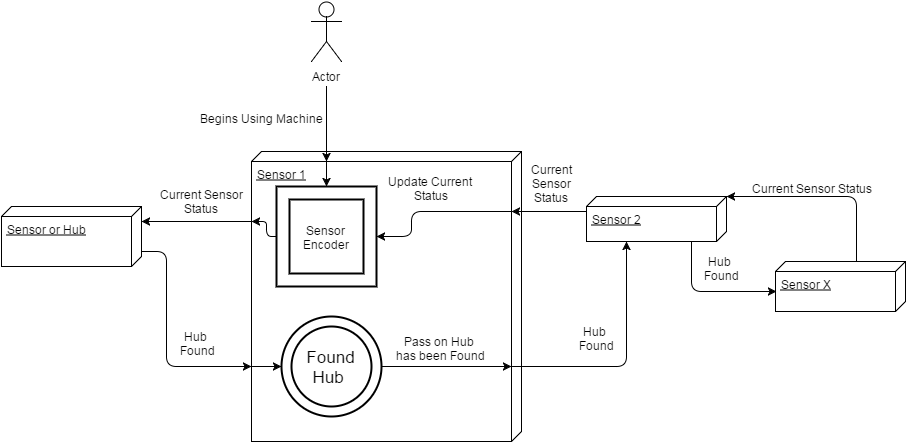
\includegraphics[width=\textwidth]{uml/sensors.png}
    \caption{UML Diagram of the Sensor Architecture}
\end{figure}

Each sensor will essentially funnel their information down to the hub through other sensors. To do this, each sensor will contain two main processes. The first process is \textit{Hub Found}. This lets other sensors further away in the funnel that the hub is "down this way". This will allow sensors, if this attribute is detected, to not continue to search for other devices to make connections to, but to focus on only one (or perhaps two for redundancy's sake) and thus conserve power. The second process is \textit{Sensor Encoder}. This process will encode the information of the sensor itself, along with the previous sensors, so that the information can be kept separate and particular to each machine. This is integral to determining which machines are in use and maintaining realistic reporting for both real-time and historic services. This process is activated by an outside actor using the equipment.

The information contained in \textit{Current Sensor Status} signal will be raw data that will be sent to the hub, and then sent on from there to the server for processing.

\subsection{Displays}

The displays are the answer to the problem of showing the user if a machine is reserved or will be reserved shortly. They also will allow the user to create a reservation locally to ensure that they will not be asked to leave the machine before they are ready to leave.


Because of the need to learn about remote reservations and push local reservations, the displays encountered a similar problem as the sensors: low power and long distance communication. With that similar problem came a similar solution: displays with mesh networking. In the figure below, one can see that the displays communicate with each other as well as the hub.

\begin{figure}[H]
    \centering
    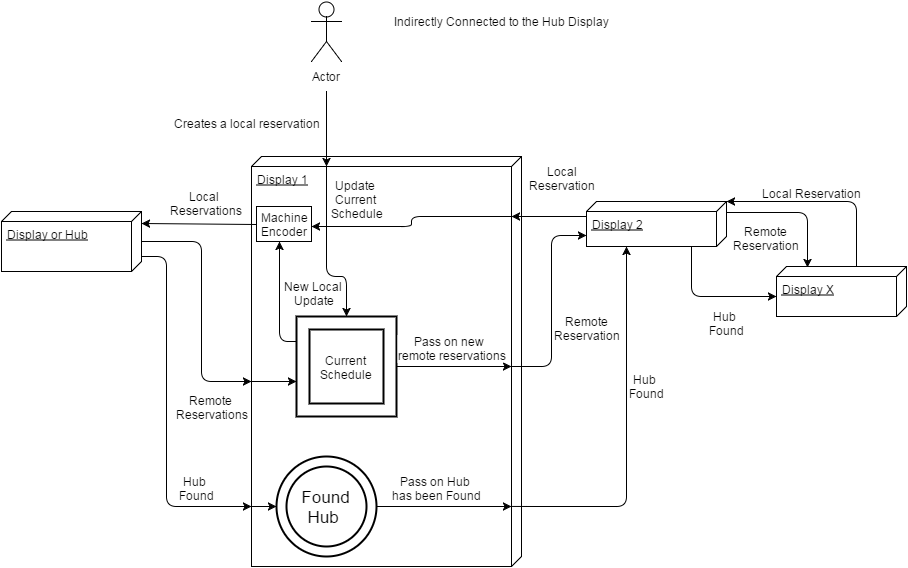
\includegraphics[width=\textwidth]{uml/displays.png}
    \caption{UML Diagram Detailing the Display Architecture}
\end{figure}

As with the sensors, the displays with funnel any information about local displays down to the hub through other displays. They will also pass a \textit{Hub Found} signal up the chain of displays to communicate when searching is not required any longer. However, displays must also retrieve information about remote reservations and thus have another connection for that.

Due to the three different streams of information, the display contains three distinct entities within itself. The first is the \textit{Hub Found} entity, which completes the same function as the \textit{Hub Found} entity within the sensors. The second entity is the \textit{Current Schedule} entity. This is essentially a basic database that contains all the information that display needs to know about its schedule. It takes in a remote reservation and decides if it is pertinent to this display. If the reservation is pertinent, it updates the current schedule. It if the reservation is not pertinent, it continues sending it up the funnel. The third entity is the \textit{Machine Encoder} which will only send information if a local reservation has been initiated by an outside actor. It will also combine any other local reservations made by machines up the funnel and then send that down the funnel, encoded in such a fashion that the hub will be able to decode which machine has new local reservations.

\subsection{Hub}

Now that all the information from the sensors and the displays has been "funneled" into the hub, the hub's first purpose is to transfer this information up to the server for processing. The other purpose is to transfer any new information to the displays, along with transferring the \textit{Hub Found} signal to the displays and sensors directly connected to the hub. This is illustrated in the figure below.

\begin{figure}[H]
    \centering
    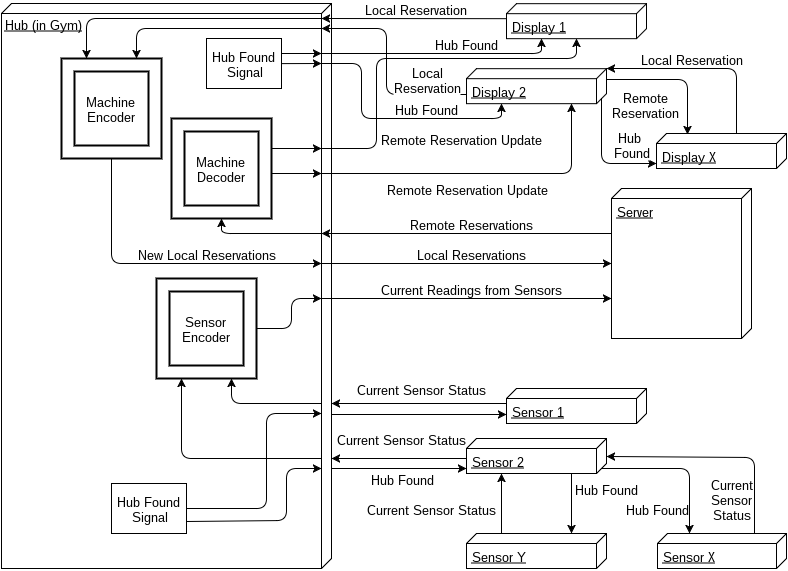
\includegraphics[width=\textwidth]{uml/hub.png}
    \caption{UML Diagram Detailing the Hub Architecture}
\end{figure}

As mentioned previously, the hub has several key processes that affect both the sensors and the displays. It must encode all of the signals that it gets from the sensors into something that it is able to send to the server for the processing of the signals. Because it can connect to several different sensors, it must have its own \textit{Sensor Encoder} that keeps track of which sensors sent which data. It is also sends a \textit{Hub Found} signal to those sensors so that they know the hub is in the current connection list.

It also handles all of the connections from the displays. Because the hub disseminates information to the different displays, it must have a \textit{Machine Decoder}, where it is able to take the information sent from the server and pass that along to the displays. It also receives information from the displays, so it must have a \textit{Machine Encoder} that takes the information received from the displays about local reservations and then passes that along to the server, so that it can maintain an up-to-date schedule. Once again, it sends a \textit{Hub Found} signal to the displays so that each display can confirm that the sensor is currently having information sent to it.

After doing all the machine encoding, the sensor makes a connection to the server which carries information about local reservations made by actors in the gym. The hub also sends the current readings from the sensors, which are encoded as well. The hub receives information about remote reservations that are made and then passes that information, after decoding it, to the displays for up-to-date displays about current schedules by machine.

\subsection{Server}

The server's main purpose is to track the information both from sensors and from remote users. It will take the information from the sensors, process the data, and then be able to display what machines are currently in use. It will pass that information to three primary locations: \textit{Current Reservation Database}, \textit{Historical Use Database}, and \textit{Current Use Database}.

The \textit{Current Reservation Database} has the most recent reservations made both locally and remotely, along with knowing if a machine is currently in use to disallow someone from reserving it out from someone's current use. Because of this it is updated from HTTP requests (from the World Wide Web actor), local reservation requests (human actor in the gym), and from current status readings (made by sensors in the gym). It then also forwards any new reservations to the machines by sending the information to the hub. This database contains all the reservations that have not yet been completed for the machines. It was created as a separate database so that sending information to the machines would be simpler and quicker, as a very large (and ever-growing) database would not have to be queried to send up-to-date information about reservations.

The \textit{Historical Use Database} simply tracks the information by machine that is received from the hub. It will act as the pool of information that administrators can draw upon to gain insight into the use of the machines and that clients will draw upon to gain health and habit insights on. It is essentially a log of all past use by machine. It will also contain information about reservations made, including if they were fulfilled, fulfilled on time, and proportion of time the machine was used with and without reservation.

The \textit{Current Use Database} is a simpler version of the Historical Use Database in that it does not log use of the past machines, but simply keeps a record of whether a machine is currently in use or not.

This system is shown in the figure below.

\begin{figure}[H]
    \centering
    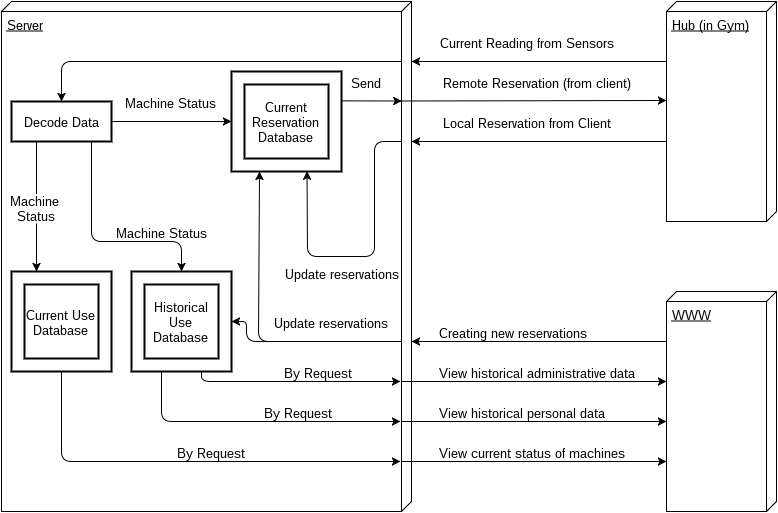
\includegraphics[width=\textwidth]{uml/server.png}
    \caption{UML Diagram Detailing the Server Architecture}
\end{figure}

The main ideas to capture from the server is that it receives current use from the hub, while sending any remote reservations gained via HTTP requests. It also logs and displays current use of the machines for personal and administrative use.

\end{document}
